%f
% programming.tex
%
% Copyright (C) 2023 UFSC.
%
% DOCUMENTATION-TEMPLATE
%
% This work is licensed under the Creative Commons Attribution-ShareAlike 4.0
% International License. To view a copy of this license,
% visit http://creativecommons.org/licenses/by-sa/4.0/.
%



\chapter{Recording to the FPGA's Internal Memory} \label{chp:chapter_rec}

    The \autoref{chp:chapter_rec} aims helping the laboratory's technician to properly configure the development board. We will first explain how to upload permanently the NEORV32, described in VHDL, to the development board.

    Then, we need to ensure that the NEORV32's toolchain is properly installed in the laboratory's computers. This toolchain provides a collection of software tools required for developing applications specifically designed for the NEORV32 processor. So, the process of downloading and installing the toolchain on the system will be presented in the following subsections:

    \autoref{sec:section_rec.1}:
    First, in this section you will find a guide on how to record the NEORV32 to the FPGA's internal memory using Intel's software, Quartus.
        
    \autoref{sec:section_rec.2}:
    Finally, we have a tutorial on how downloading and installing the toolchain.
    
    \section{Step by step to record in internal memory} \label{sec:section_rec.1}
    
        First, open the .sof to .pof (programming object file) converter. To do that, you should go to File > Convert Programming Files. Then you will have access to the window presented in \autoref{fig:f1}).

            \begin{figure}[!ht]
                \begin{center}
                    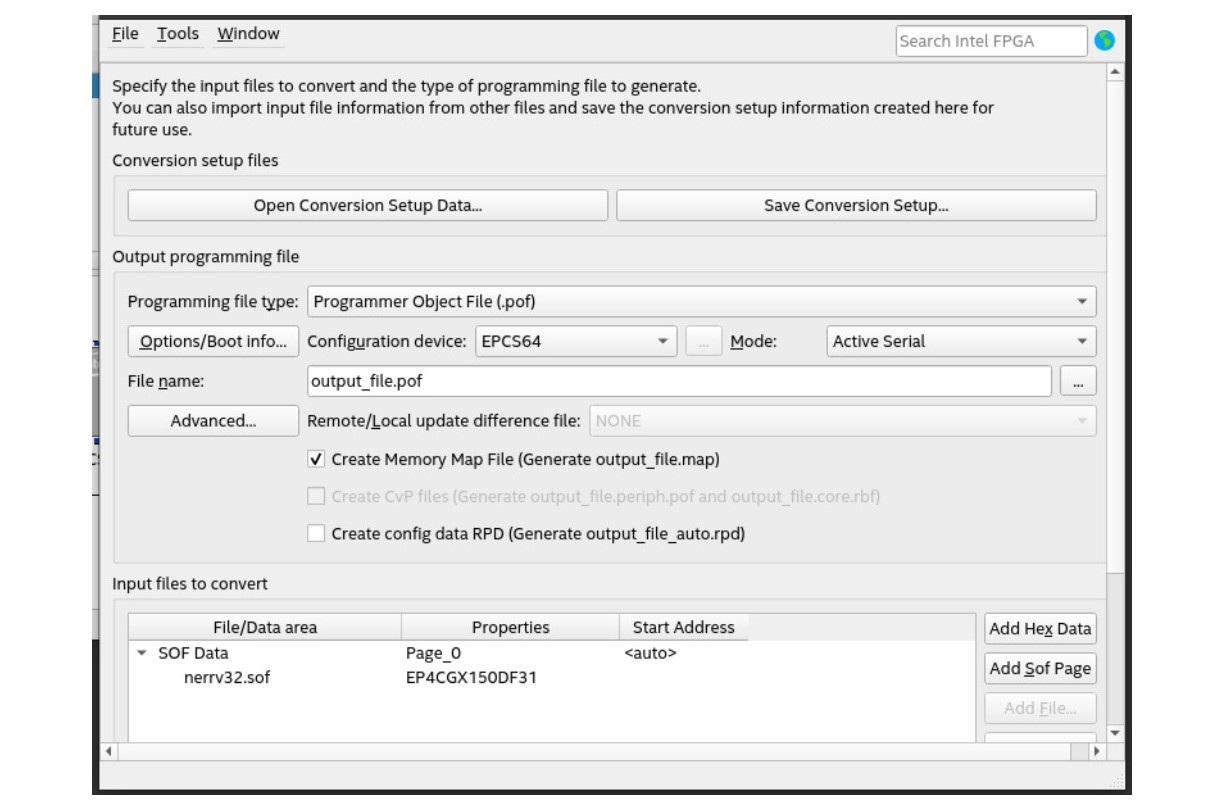
\includegraphics[width= 0.8\textwidth]{figures/chap2/fpga1.jpg}
                    \caption{\label{fig:f1} Convert Programming Files Tool.}
                \end{center}
            \end{figure}        
            
        Then, on the development board switch to the recording mode (PROG) using the ``programming mode switch'', shown in the \autoref{fig:f2}.
        
            \begin{figure}[!ht]
                \begin{center}
                    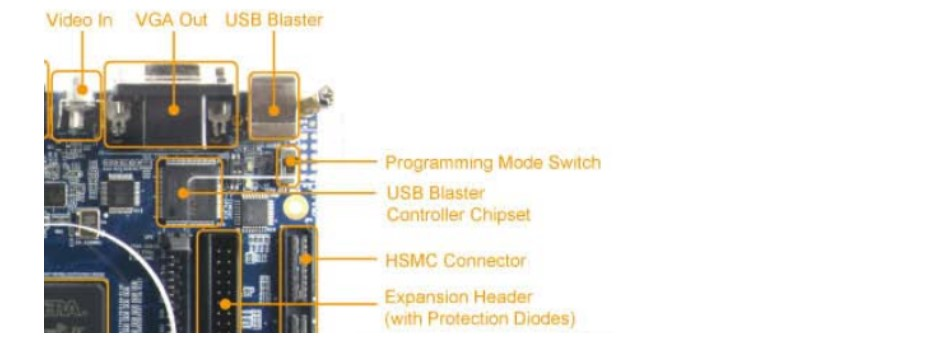
\includegraphics[width= 0.7\textwidth]{figures/chap2/fpga2.jpg}
                    \caption{\label{fig:f2} Programming Switch Indication.}
                \end{center}
            \end{figure}
        
        Next, on Quartus II, go to Tools > Programmer.
            
            \begin{figure}[!ht]
                \begin{center}
                    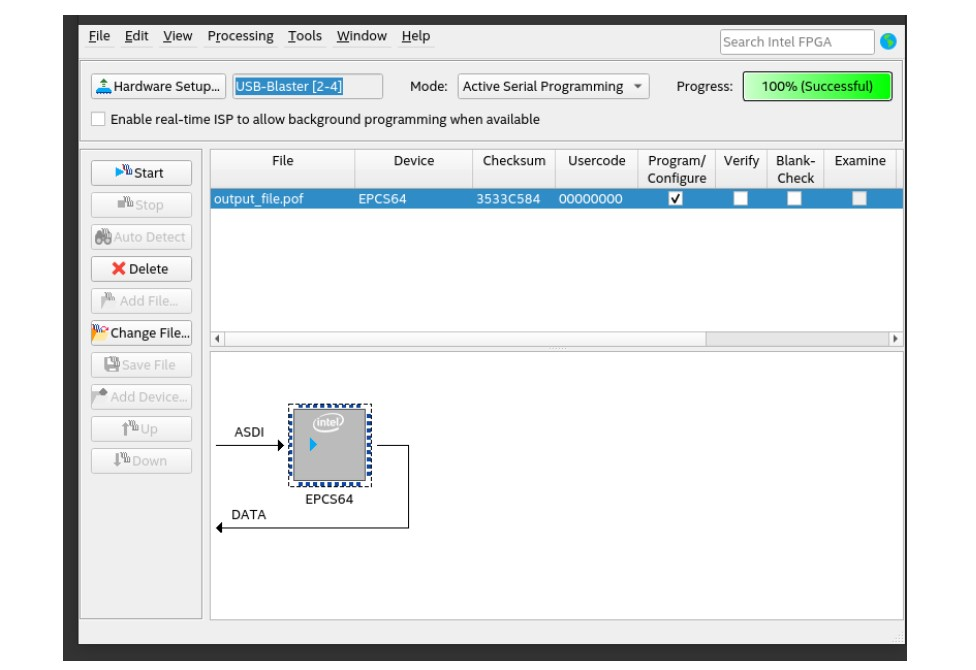
\includegraphics[width= 0.8\textwidth]{figures/chap2/fpga3.jpg}
                    \caption{\label{fig:f3} Programmer Tool.}
                \end{center}
            \end{figure}
        
        Finally, set the mode to ``active serial programming'', add the .pof file and click start, as presented in \autoref{fig:f3}. Before starting the development board, return the mode to ``run''.

        \section{Downloading and installing the toolchain} \label{sec:section_rec.2}
    
            First, you should access \url{https://github.com/stnolting/riscv-gcc-prebuilt}, to download the most recent available toolchain (today, \today, \textcolor{blue}{\textbf{rv32i-4.0.0}}). You should have now access to a .tar.gz file. Then, the next step, is to create the folder that the toolchain is going to be installed. You can open a terminal and type:
            
                \begin{lstlisting}[style=mystyle_bash, language=bash]
                    $ sudo mkdir /opt/riscv
                \end{lstlisting}
            
            Now, you need to navigate to the folder where the .tar.gz file was downloaded, like:
            
                \begin{lstlisting}[style=mystyle_bash, language=bash]
                    $ cd Downloads/
                \end{lstlisting}
                
            And then you have to extract the .tar.gz file to the folder previously created:
            
                \begin{lstlisting}[style=mystyle_bash, language=bash]
                    $ sudo tar -xzf <toolchain_version>.tar.gz -C /opt/riscv/
                \end{lstlisting}
                
            Finally, you should add the toolchain's bin folder to your system's PATH environment variable. You can open the .bashrc file:
            
                \begin{lstlisting}[style=mystyle_bash, language=bash]
                    $ sudo nano .bashrc
                \end{lstlisting}
                
            And then add the following line in the end of the .bashrc file:
            
                \begin{lstlisting}[style=mystyle_bash, language=bash]
                    export PATH="/opt/riscv/bin:$PATH"
                \end{lstlisting}
                
            To make sure everything works fine, navigate to the folder with the aplication examples and execute the following command:
            
                \begin{lstlisting}[style=mystyle_bash, language=bash]
                    $ make check
                \end{lstlisting}
            
            If everything is working fine you should se an ``\textbf{OK}'' appearing at the end, like in the \autoref{fig:successful_check}.
            
                \begin{figure}[!ht]
                    \begin{center}
                        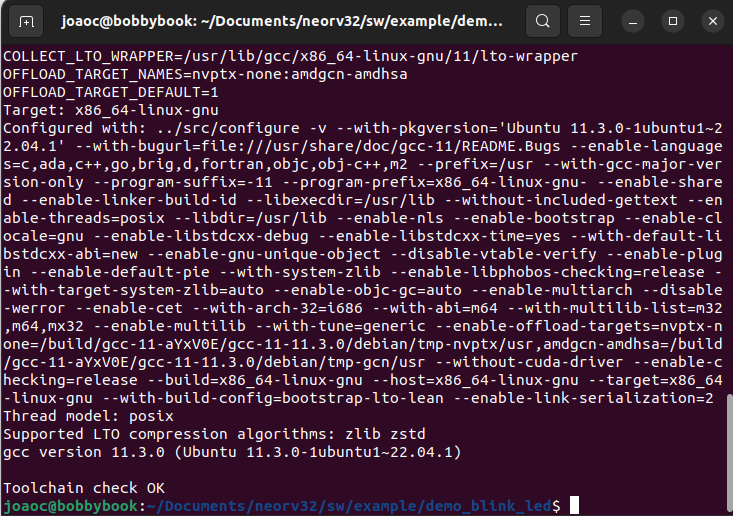
\includegraphics[width= 0.6\textwidth]{figures/successful_check.png}
                        \caption{Indication that the installation was successful.}
                        \label{fig:successful_check}
                    \end{center}
                \end{figure}
        

\chapter{Compiling and executing your first program} \label{ch:chapter_comp}

    Now, we will explore the process of compiling and executing your first program using the NEORV32's toolchain. This chapter aims to guide you through the necessary steps to successfully compile and run programs on the NEORV32.
    
    \autoref{sec:section_comp.1}: In this section, we will explore the process of flashing the compiled program into the FPGA board using the NEORV32 bootloader. The bootloader serves as an intermediary step between the development environment and the execution of the program on the FPGA board. We will guide you through the steps required to configure a terminal emulator, communicate with the FPGA board, and upload the program for execution.
    
    \autoref{sec:section_comp.2}: In addition to using the bootloader, we will also discuss an alternative method for flashing programs directly onto the FPGA board. This approach servers only to those that want to try something different, but it is no recommended using it during the course. It involves generating a VHDL file (.vhd) that represents the application code to be stored in the Instruction Memory (IMEM) of the NEORV32 processor. We will explain how to generate the .vhd file and integrate it into your project, either by replacing the existing application file or adding it to the project if it does not already exist.
    
    By understanding the process of compiling and executing programs on the NEORV32 processor and FPGA board, both you and your students will gain valuable practical experience in working with embedded systems. So, let's dive into the exciting world of FPGA programming and explore the possibilities offered by the NEORV32 toolchain!
    
    
    
        %\subsection{Some important commands}
        
        %Now that the toolchain was installed, you should know some commands to generate the .hex, .bin, .vdh, as well as other types of files. As you can see in \autoref{fig:toolchain_commands}, you could use \texttt{\hl{hex}} to generate the .hex file, which represents the machine language. You could use, for instance, the \texttt{\hl{image}} to generate the .vhd file, which is used to generate the \textit{neor32\_application\_image.vhd} that stores the main program that will run in the microprocessor. 
        
        
        %\begin{figure}[!ht]
        %    \begin{center}
        %        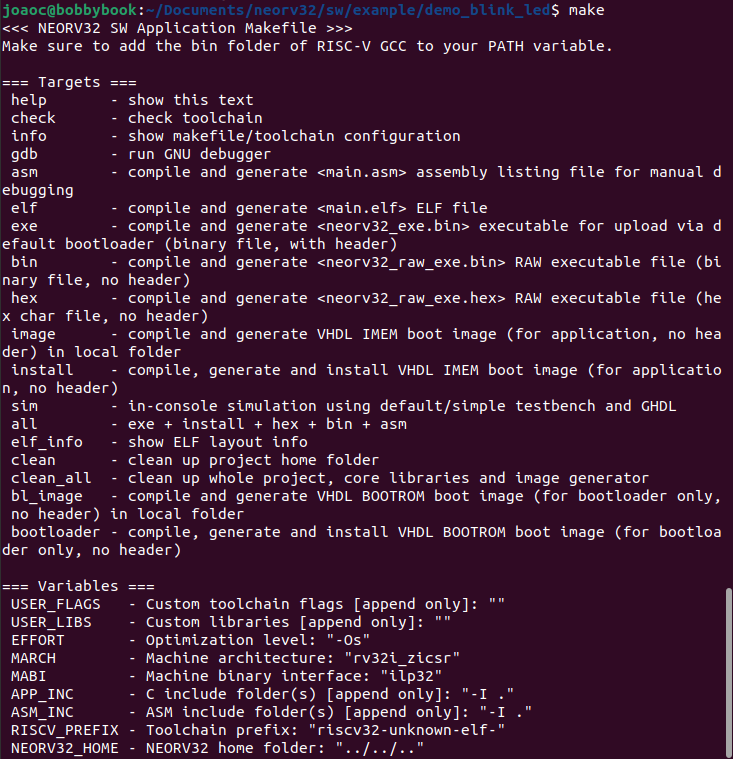
\includegraphics[width= 0.6\textwidth]{figures/toolchain_commands.png}
        %        \caption{Some useful commands to use.}
        %        \label{fig:toolchain_commands}
        %    \end{center}
        %\end{figure}
        
    \section{Flash the program into FPGA Board using bootloader} \label{sec:section_comp.1}
    
        In Linux, you should install a terminal emulator, like Minicom, Cutecom or similar:
        
            \begin{lstlisting}[style=mystyle_bash, language=bash]
                $ sudo apt install cutecom
            \end{lstlisting}
        
        Then the software should be configured like in \autoref{fig:cutecom_configuration}.  With the FPGA previously programmed with the base of the NEORV32, you should see the status LED (LDEG[0]) starts blinking and the bootloader intro screen appearing in your console, like:
        
            \begin{lstlisting}[style=mystyle_bash, language=bash]
                << NEORV32 Bootloader >>
            
                BLDV: Mar  7 2023
                HWV:  0x01080107
                CID:  0x00000000
                CLK:  0x05f5e100
                MISA: 0x40901106
                XISA: 0xc0000fab
                SOC:  0xffff402f
                IMEM: 0x00008000 bytes @0x00000000
                DMEM: 0x00002000 bytes @0x80000000
            
                Autoboot in 8s. Press any key to abort.
            \end{lstlisting}
            
            \begin{figure}[!ht]
                \begin{center}
                    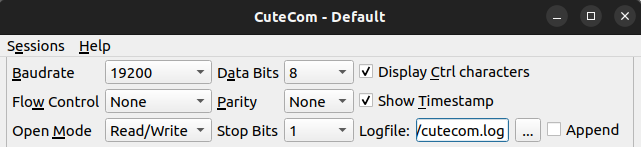
\includegraphics[width= 0.6\textwidth]{figures/cutecom_configuration.png}
                    \caption{Cutecom configuration.}
                    \label{fig:cutecom_configuration}
                \end{center}
            \end{figure}
            
        Now you can press any key to abort the automatic boot sequence and to start the actual bootloader user interface console. You then will have access to some commands, like:
        
            \begin{lstlisting}[style=mystyle_bash, language=bash]
                Available CMDs:
                h: Help
                r: Restart
                u: Upload
                s: Store to flash
                l: Load from flash
                x: Boot from flash (XIP)
                e: Execute
            \end{lstlisting}
        
        You can now upload the .bin file to execute it in the NEORV32. First you should create this file, by going to your application's folder and compiling it: 
        
            \begin{lstlisting}[style=mystyle_bash, language=bash]
                $ make clean_all exe
            \end{lstlisting}
    
        This command will create the \textit{neorv32\_exe.bin} file, which you will send to the FPGA. Then click on the \textit{send file} option to select the correct file. Finally, you can execute the program.
        
    \section{Flash the program into FPGA board directly} \label{sec:section_comp.2}
        
        To generate an .vhd file for the IMEM that contains the actual application, run the \texttt{\hl{image}} inside the folder of your application. For instance, you could use any application from the NEORV32's examples folder, like neorv32-setup/sw/exmaple/demo\_blink\_led:
        
            \begin{lstlisting}[style=mystyle_bash, language=bash]
                $ make clean_all image
            \end{lstlisting}
        
        This command will create the \textit{neorv32\_application\_image.vhd} file, that you can then add to the project's folder. If you are using Quartus II, you could replace the current application file or add it to the project if don't exists already.